\documentclass[xcolor={dvipsnames, svgnames, x11names, table}, 10pt]{beamer}
\usepackage{./assets/preamble}

\title{Programmazione generica e \texttt{STL}}
\date{5 ottobre 2021}
\institute{%
    \textbf{Obiettivi di apprendimento}:
    \begin{itemize}
        \item Operazioni sulle liste;
        \item TODO;
        \item TODO.
    \end{itemize}%
}

% arara: xelatex: { synctex: no }
% arara: xelatex: { synctex: yes }
% arara: latexmk: { clean: partial }
\begin{document}

\frame{\titlepage}

\section*{Riassunto lezione precedente}

\begin{frame}{Argomenti trattati nell'ultima lezione}

    \begin{itemize}
        \item Programmazione generica, template e introduzione STL;
        \item STL: esempi di uso contentitori.
    \end{itemize}

\end{frame}

\section{Contenitori}

\begin{frame}{Contenitori}

    \begin{itemize}
        \item sono Template che \enquote{contengono} altri tipi parametrici;
        \item il contenuto si accede usando gli iterativi.
    \end{itemize}

\end{frame}

\begin{frame}[c]{Iteratori}

    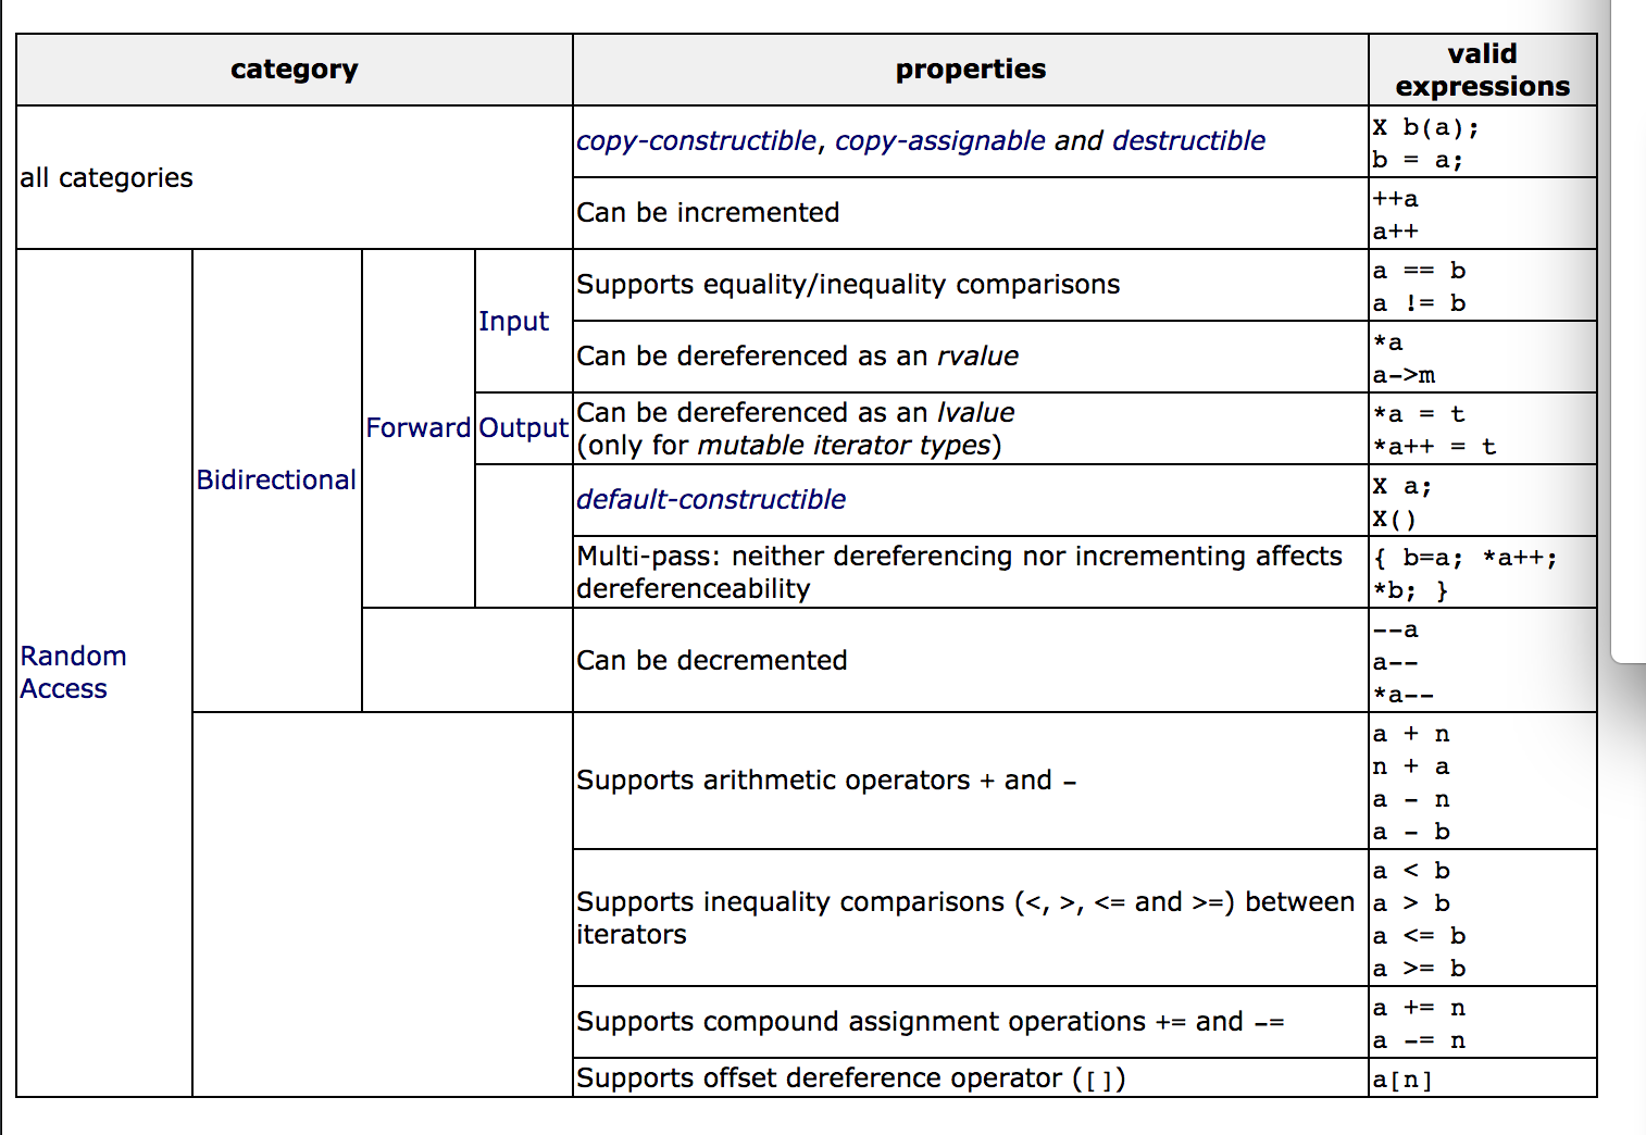
\includegraphics[width=\textwidth, trim={0.2cm 0.55cm 0.75cm 0.5cm}, clip]{iterators}

\end{frame}

\begin{frame}[label=listone, t, fragile]{list [1/6]}

    \only<1>{\cppfilepath[lastline=9, highlightlines={1-2,6}]{Esempio0/main.cpp}}
    \only<2>{\cppfilepath[lastline=9, highlightlines={4}]{Esempio0/main.cpp}}
    \only<3>{\cppfilepath[lastline=9, highlightlines={8-9}]{Esempio0/main.cpp}}

\end{frame}

\begin{frame}[label=listtwo, t, fragile]{list [2/7]}

    \only<1>{\cppfilepath[firstline=11, lastline=28, highlightlines={11-12}]{Esempio0/main.cpp}}
    \only<2>{\cppfilepath[firstline=11, lastline=28, highlightlines={14-16}]{Esempio0/main.cpp}}
    \only<3>{\cppfilepath[firstline=11, lastline=28, highlightlines={18-19}]{Esempio0/main.cpp}}
    \only<4>{\cppfilepath[firstline=11, lastline=28, highlightlines={21-22}]{Esempio0/main.cpp}}
    \only<5>{\cppfilepath[firstline=11, lastline=28, highlightlines={24-25}]{Esempio0/main.cpp}}
    \only<6>{\cppfilepath[firstline=11, lastline=28, highlightlines={27-28}]{Esempio0/main.cpp}}
    
    \begin{center}
        \uncover<2->{\texttt{32}}\uncover<3->{\texttt{32}}\uncover<4->{\texttt{32}}\uncover<6->{\texttt{43}}
    \end{center}

\end{frame}

\begin{frame}[label=listthree, t, fragile]{list [3/6]}

\begin{columns}[c]
    
\column{0.55\textwidth}
    \only<01>{\cppfilepath[firstline=33, lastline=56, highlightlines={33}]{Esempio0/main.cpp}}
    \only<02>{\cppfilepath[firstline=33, lastline=56, highlightlines={34}]{Esempio0/main.cpp}}
    \only<03>{\cppfilepath[firstline=33, lastline=56, highlightlines={36-38}]{Esempio0/main.cpp}}
    \only<04>{\cppfilepath[firstline=33, lastline=56, highlightlines={39-40}]{Esempio0/main.cpp}}
    \only<05>{\cppfilepath[firstline=33, lastline=56, highlightlines={42-44}]{Esempio0/main.cpp}}
    \only<06>{\cppfilepath[firstline=33, lastline=56, highlightlines={45-46}]{Esempio0/main.cpp}}
    \only<07>{\cppfilepath[firstline=33, lastline=56, highlightlines={48-49}]{Esempio0/main.cpp}}
    \only<08>{\cppfilepath[firstline=33, lastline=56, highlightlines={50-51}]{Esempio0/main.cpp}}
    \only<09>{\cppfilepath[firstline=33, lastline=56, highlightlines={53-54}]{Esempio0/main.cpp}}
    \only<10>{\cppfilepath[firstline=33, lastline=56, highlightlines={55-56}]{Esempio0/main.cpp}}

\column{0.45\textwidth}
    \uncover<1->{\texttt{4}}%
    \uncover<2->{\texttt{3}}
    
    \uncover<4->{\texttt{5432}}
    
    \uncover<6->{\texttt{43}}
    
    \uncover<8->{\texttt{743}}
    
    \uncover<10->{\texttt{743743}}
    
\end{columns}

\end{frame}

\begin{frame}[t, fragile]{list [4/6]}

\begin{columns}[c]
    
\column{0.7\textwidth}
    \only<1>{\cppfilepath[firstline=61, lastline=84, highlightlines={61}]{Esempio0/main.cpp}}
    \only<2>{\cppfilepath[firstline=61, lastline=84, highlightlines={62-63}]{Esempio0/main.cpp}}
    \only<3>{\cppfilepath[firstline=61, lastline=84, highlightlines={64-66}]{Esempio0/main.cpp}}
    \only<4>{\cppfilepath[firstline=61, lastline=84, highlightlines={67}]{Esempio0/main.cpp}}
    \only<5>{\cppfilepath[firstline=61, lastline=84, highlightlines={69-70}]{Esempio0/main.cpp}}
    \only<6>{\cppfilepath[firstline=61, lastline=84, highlightlines={71-73}]{Esempio0/main.cpp}}
    \only<7>{\cppfilepath[firstline=61, lastline=84, highlightlines={74-76}]{Esempio0/main.cpp}}
    \only<8>{\cppfilepath[firstline=61, lastline=84, highlightlines={78}]{Esempio0/main.cpp}}
    \only<9>{\cppfilepath[firstline=61, lastline=84, highlightlines={79-81}]{Esempio0/main.cpp}}
    \only<10>{\cppfilepath[firstline=61, lastline=84, highlightlines={82-84}]{Esempio0/main.cpp}}

\column{0.3\textwidth}
    \uncover<3->{\texttt{l:98743743}}
    
    \uncover<4->{\texttt{7}}
    
    \uncover<6->{\texttt{l:98}}\\
    \uncover<7->{\texttt{l2:743743}}
    
    \uncover<9->{\texttt{l:743743}}\\
    \uncover<10->{\texttt{l2:98}}
    
\end{columns}

\end{frame}

\begin{frame}[label=current, t, fragile]{list [5/6]}

\begin{columns}[c]
    
\column{0.7\textwidth}
    \only<1>{\cppfilepath[firstline=88, lastline=108, highlightlines={88}]{Esempio0/main.cpp}}
    \only<2>{\cppfilepath[firstline=88, lastline=108, highlightlines={89}]{Esempio0/main.cpp}}
    \only<3>{\cppfilepath[firstline=88, lastline=108, highlightlines={91-93}]{Esempio0/main.cpp}}
    \only<4>{\cppfilepath[firstline=88, lastline=108, highlightlines={95-97}]{Esempio0/main.cpp}}
    \only<5>{\cppfilepath[firstline=88, lastline=108, highlightlines={99-101}]{Esempio0/main.cpp}}
    \only<6>{\cppfilepath[firstline=88, lastline=108, highlightlines={103}]{Esempio0/main.cpp}}
    \only<7>{\cppfilepath[firstline=88, lastline=108, highlightlines={104}]{Esempio0/main.cpp}}
    \only<8>{\cppfilepath[firstline=88, lastline=108, highlightlines={105-106}]{Esempio0/main.cpp}}
    \only<9>{\cppfilepath[firstline=88, lastline=108, highlightlines={107-108}]{Esempio0/main.cpp}}

\column{0.3\textwidth}
    \uncover<1->{\texttt{6}}%
    \uncover<2->{\texttt{0}}
    
    \uncover<3->{\texttt{l:347347}}\\
    \uncover<4->{\texttt{l:334477}}\\
    \uncover<5->{\texttt{l:347}}
    
    \uncover<8->{\texttt{l:34789}}\\
    \uncover<9->{\texttt{l2:}}
    
\end{columns}

\end{frame}

\begin{frame}[t, fragile]{list [5/6]}

\begin{columns}[c]
    
\column{0.7\textwidth}
    \only<1>{\cppfilepath[firstline=113, lastline=136, highlightlines={113-115}]{Esempio0/main.cpp}}
    \only<2>{\cppfilepath[firstline=113, lastline=136, highlightlines={117-118}]{Esempio0/main.cpp}}
    \only<3>{\cppfilepath[firstline=113, lastline=136, highlightlines={120-121}]{Esempio0/main.cpp}}
    \only<4>{\cppfilepath[firstline=113, lastline=136, highlightlines={123-124}]{Esempio0/main.cpp}}
    \only<5>{\cppfilepath[firstline=113, lastline=136, highlightlines={126-127}]{Esempio0/main.cpp}}
    \only<6>{\cppfilepath[firstline=113, lastline=136, highlightlines={129-130}]{Esempio0/main.cpp}}
    \only<7>{\cppfilepath[firstline=113, lastline=136, highlightlines={132-133}]{Esempio0/main.cpp}}
    \only<8>{\cppfilepath[firstline=113, lastline=136, highlightlines={135-136}]{Esempio0/main.cpp}}

\column{0.3\textwidth}
    
\end{columns}

\end{frame}

\begin{frame}[t, fragile]{list [6/6]}

\begin{columns}
    
\column{0.7\textwidth}
    \cppfilepath[firstline=111, lastline=121]{Esempio0/main1-original.cpp}

\column{0.3\textwidth}
    
\end{columns}

\end{frame}

\begin{frame}{Operazioni non viste sulle liste}
    
    \begin{itemize}
        \item \textbf{\texttt{emplace\_front}}
        \item \textbf{\texttt{emplace\_back}}
        \item \textbf{\texttt{set\_allocator}}
        \item \textbf{\texttt{crbegin}}
        \item \textbf{\texttt{crend}}
    \end{itemize}
    
\end{frame}

\section{Set e Map}

\begin{frame}[t, fragile]{Set e map}

\begin{itemize}
    \item Sono ordinati e usano \texttt{operator<};
    \item \textbf{non} hanno il concetto di \enquote{front} e \enquote{back};
    \item si usa \texttt{insert}
\end{itemize}

\begin{minted}[numberblanklines = false]{cpp}
Class A{ };

set<A> s;

s.insert(A()); // funziona solo se definito A::operator<

map<A,int> m;

m.insert(pair<A,int> (A(),2));
// funziona solo se definito A::operator<

map<int,A> ma;

ma.insert(pair<int,A> (3,A()));
// funziona, operator< definito per gli int tipo base

ma[3] = A(); // equivalentemente per il map è ridefinito operator[]
\end{minted}

\end{frame}

\subsection{Esempio con codice}

\begin{frame}{\texttt{film.h}}
    
\cppfilepath[]{Esempio1/film.h}
    
\end{frame}

\begin{frame}{\texttt{film.cpp}}
    
\cppfilepath[]{Esempio1/film.h}
    
\end{frame}

\subsection{Esempio con codice}

\begin{frame}{\texttt{spettatore.h}}
    
\cppfilepath[]{Esempio1/film.h}
    
\end{frame}

\begin{frame}{\texttt{spettatore.cpp}}
    
\cppfilepath[]{Esempio1/film.h}
    
\end{frame}

\begin{frame}{\texttt{cineteca.h}}
    
\cppfilepath[]{Esempio1/film.h}
    
\end{frame}

\begin{frame}{\texttt{cineteca.cpp}}
    
\cppfilepath[]{Esempio1/film.h}
    
\end{frame}

\begin{frame}{\texttt{main.cpp}}
    
\cppfilepath[]{Esempio1/main.cpp}
    
\end{frame}


\section{Multiset e multimap}

\begin{frame}[fragile]{Multiset e multimap}

Come set e map ma permettendo valori multipli

nel multimap non c'é operator[]

\end{frame}

\subsection{Esempio con codice}

\begin{frame}{\texttt{fraction.h}}

\cppfilepath[]{Esempio1/fraction.h}
    
\end{frame}

\begin{frame}{\texttt{fraction.cpp}}
    
\cppfilepath[]{Esempio1/fraction.cpp}
    
\end{frame}

\Riconoscimenti

\end{document}